\documentclass[10pt,a4paper,fleqn,dvipdfmx]{jsarticle}
\usepackage{graphicx}
\usepackage{amsmath,amssymb}

\begin{document}

\begin{center}

{\Large レポートのサンプル}

\vspace{2mm}
00TI0000 AAAA BBBB

\vspace{2mm}
20@@年@@月@@日 提出
\end{center}

以下に,書き方の例を示す.
あくまで例なので,各自で書きやすいよう,適宜形式を変更すること.
ただし,「目的」「方法」「結果」「考察」の内容を必ず入れること.

\section{目的}

- 本課題の目的を説明する.\\
 \qquad 例) ○○のデータを使って,□□と●●の関係を解析し,考察する.

\section{方法・結果}

- 扱ったデータについて説明する.
\begin{quote}
例) data.csvの変数\\
\ \ \ \ \ ○○○:気温 (℃)\\
\ \ \ \ \ △△△:湿度 ($\%$)
\end{quote}

- 何をするかを説明する.
\begin{quote}
例) ○○を目的変数に,△△を説明変数として線形回帰を行う.
\end{quote}

- 何を得られたかを説明する.
\begin{quote}
例) 線形回帰をした結果,$R^2$スコアとして 0.67 の数値が得られた.各変数の係数として [$\cdots$] が得られた.
\end{quote}

\section{考察}

- 結果から何が言えるかを説明する.
\begin{quote}
例) 「気温」の係数が大きくなったことから,「アイスクリームの売上」には「気温」が大きく関係していることがわかる.
$R^2$スコアが低いことから,十分な線形回帰近似を行えていない.○○をすることでより精度が向上すると考えられる.
\end{quote}

\subsection{図の貼り付け方について}

図~\ref{fig_sample}は〜を示す.

\begin{figure}[htb]
\begin{center}
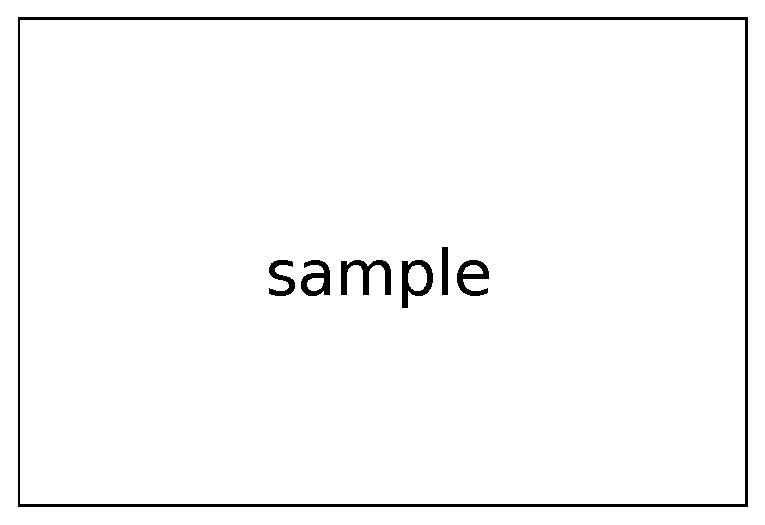
\includegraphics[width=60mm]{sample.eps}
\caption{サンプル.}
\label{fig_sample}
\end{center}
\end{figure}


\section{まとめ}

まとめ.


\end{document}
